\documentclass[11pt]{article}
\usepackage{amsmath,amssymb,amsthm}
\usepackage{graphicx}
\usepackage[margin=1in]{geometry}
\usepackage{fancyhdr}
\usepackage{float}
\setlength{\parindent}{0pt}
\setlength{\parskip}{5pt plus 1pt}
\setlength{\headheight}{13.6pt}
\newcommand\question[2]{\vspace{.25in}\hrule\textbf{#1: #2}\vspace{.5em}\hrule\vspace{.10in}}
\renewcommand\part[1]{\vspace{.10in}\textbf{(#1)}}
\newcommand\algorithm{\vspace{.10in}\textbf{Algorithm: }}
\newcommand\result{\vspace{.10in}\textbf{Result: }}
\pagestyle{fancyplain}
\lhead{\textbf{\NAME\ (\ANDREWID)}}
\chead{\textbf{Assignment\HWNUM}}
\rhead{STAT3006: Statistical Computing}
\begin{document}\raggedright
%Section A==============Change the values below to match your information==================
\newcommand\NAME{ZHANG Xinfang}  % your name
\newcommand\ANDREWID{1155141566}     % your student id
\newcommand\HWNUM{2}              % the homework number
%Section B==============Put your answers to the questions below here=======================

\question{1}{Inverse method for Poissson Distribution (25\%)} 
For discrete Poisson Distribution ($\lambda = 5$),

the p.m.f is $P(x|\lambda) = e^{-\lambda} \frac{\lambda^x}{x!}$ and
the c.d.f is $F(x|\lambda) = \sum_{t \leq x} e^{-\lambda} \frac{\lambda^t}{t!}$.

\algorithm
Inverse method for the Poisson Distribution:

To generate $X \sim F(x)$:

STEP 1: Generate $U \sim unif[0, 1]$;

STEP 2: Transform $X = F^-(U)$: if $F(x|\lambda) < U \leq F(x+1|\lambda)$, let $X = x+1$.

$\mathbf{Plot:}$

\begin{figure}[H]
    \centering
    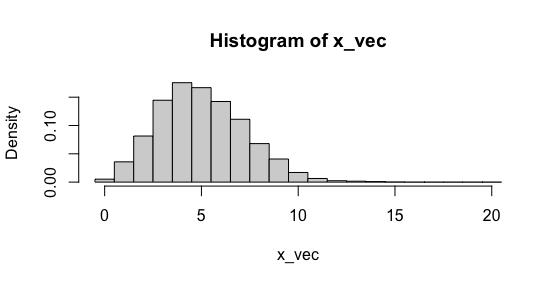
\includegraphics[width=15cm]{figures/q1_plot.png}
    \caption{Histogram of 5000 samples}
  \end{figure}
\question{2}{Accept-Reject method for truncated Gamma Distribution(25\%)}

\part{1} 

\part{2}

\question{3}{Importance Sampling for Estimation(25\%)}

\part{1} 

\part{2}

\algorithm

\result

\question{4}{Stratified Sampling25\%)}

\part{1} 

\part{2}

\part{3} 

\end{document}
